\chapter{Introduction}
\begin{figure}[H]
        \centering
        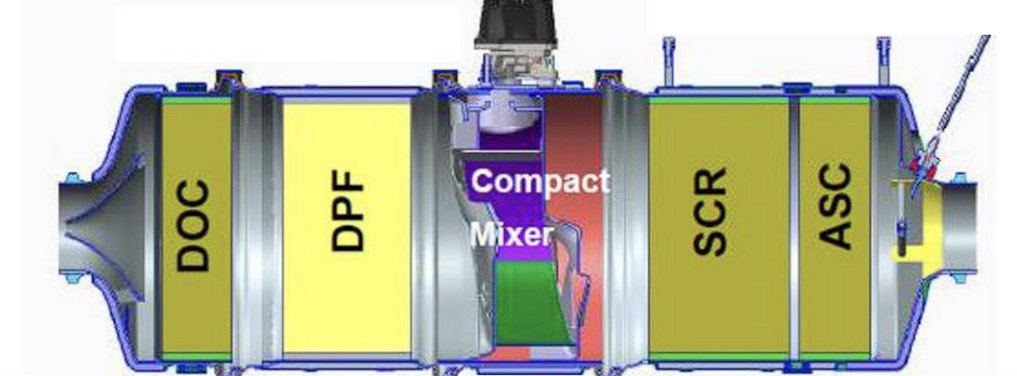
\includegraphics[width = 0.7\textwidth]{Part3/figs/SCR-ASC_chamber.png}
        \caption{Diesel Engine SCR-ASC System}
        \label{fig::scr_chamber}
\end{figure}

Modern Diesel after-treatment systems with Selective Catalytic Reduction (SCR) - Ammonia Slip Catalyst (ASC) need
on-board diagnostics (OBD) tools that can accurately report SCR degradation level while avoiding false pass and false
fail. The diagnostic tool's performance must contain the following features: 1) high estimation accuracy; 2) high
robustness against various noise factors under harsh on-road operating conditions; 3) minimal negative impact on SCR
emissions control; and 4) cost-effective by using existing SCR configurations and commercially available $NO_x$ sensors.
Since it is very difficult to imitate real-world catalyst degradation using test-cell accelerated aging, none of the
existing control-oriented SCR-aging models have been validated or tested on real-world catalyst degradation data.
Numerous studies have been conducted on modeling the SCR-ASC systems and their control (\cite{yuan2015diesel}). A
prevalent modeling approach is to approximate the PDE (partial differential equation) model from the plug flow reactor
assumption into a set of ODEs (ordinary differential equations) using the idealization of the plug-flow reactor into a
sequence of continuous stirred tank reactors (CSTRs) (\cite{hsieh2011development}, and \cite{nova2014urea}). This
discretization requires at least 2 CSTRs to capture the system dynamics and causality, thereby increasing the model
order. Moreover, the reactions considered are generally confined to selected SCR and ASC reactions. The single CSTR
approach was first justified in \cite{devarakonda2008adequacy} and a nonlinear model was developed using these
assumptions, which was then linearized for feedback control design (\cite{devarakonda2009model}). With this model,
observers were designed to estimate the states corresponding to the catalyst's storage (\cite{ma2017observer},
\cite{jain2020term}). A method for detecting the catalyst's aging by observing the change in the maximum storage
capacity of the catalyst, modeled as an exponential function of temperature, was also proposed in \cite{ma2017observer}.
A common theme in these studies is the non-uniqueness in estimating the nonlinear parameters without a priori
constraints on the actual values. Moreover, these studies assume the availability of all the gaseous states at tail-pipe
to eliminate the effects of cross-sensitivity of the $NO_x$ sensors, which is not always the case in real-world
applications. Another limitation of existing OBD methods for SCR systems is that they do not consider the presence of
Ammonia Slip Catalyst (ASC) in series with SCR. Also, most existing OBD approaches cannot work under the limitations of
commercial after-treatment instrumentation such as unavailability of $NH_3$ sensors, cross-sensitive $NO_x$ sensors,
etc.

Therefore, development of better models to design OBD methods that can work with commercial systems under on-road
conditions is required. Out goal is to fill this research gap by investigating model-based diagnostic algorithms to
detect aging in SCR systems. The overall research endeavor includes:

\begin{enumerate}
\item achieving insight in SCR aging from modeling and diagnostic perspectives via the comprehensive analysis of
experimental data;
\item developing accurate control-oriented after-treatment models to predict reduced emissions systems' performance at
different degradation levels, and
\item developing robust and effective non-intrusive diagnostic methods that could distinguish SCR catalysts at different
aging levels for real-world driving conditions.
\end{enumerate}

As part of this effort, Cummins provided real-world truck data and test-cell data. Our approach is based on the presumption that the aging detection can be framed as a state/parameter estimation problem with respect to the concentration dynamics of the gases involved. This gives rise to the following sub-problems:

\begin{enumerate}
\item Determining a suitable model for the system dynamics.
\item Assessing whether the available data contains sufficient information for identifying the model parameters related to the chosen system dynamics.
\item Investigating the relationship between the parameters/states and the aging
factor of the catalyst. And, designing the relevant estimation algorithms.
\item Understanding the uncertainties inherent in the aforementioned processes.
\item Finally, developing and validating the aging detection algorithm.
\end{enumerate}
